\documentclass[12pt,a4paper, titlepage]{article}
\usepackage[latin1]{inputenc}
\usepackage{amsmath}
\usepackage{amsfonts}
\usepackage{amssymb}
\usepackage{graphicx}
\usepackage{glossaries}
\usepackage{bm}
\usepackage{mathtools}
\usepackage{enumerate}
\usepackage{tikz}
\usetikzlibrary{arrows}
\usetikzlibrary{bayesnet}
\usepackage{caption}
\usepackage{url}
\usepackage[noabbrev]{cleveref}
%Double spacing
\usepackage{setspace}
\onehalfspacing

\newcommand{\rhat}{\widehat{R}}

\usepackage[left=2.00cm, right=2.00cm, top=2.00cm, bottom=2.00cm]{geometry}
\author{Demetri Pananos}
\title{Doctoral Thesis Research Proposal}
\begin{document}
	
	\pagenumbering{roman}
	\maketitle
	\tableofcontents
	\setcounter{tocdepth}{5}
	\setcounter{secnumdepth}{2}
	\newpage
	
	%Reset page numbers
	\pagenumbering{gobble}% Remove page numbers (and reset to 1)
	\pagenumbering{arabic}
	
	
	%Inlcude sections here
	\section{Introduction}
	
	\newpage
	\section{Literature Review}
	\subsection{Differential Equations}

In this section, I discuss elements of differential equation theory.  I begin by delineating between different types of differential equations.  I then discuss sufficient conditions for existence and uniqueness of solutions to differential equations, followed by a discussion of computing analytic representations of said solutions.  I conclude this section with numerical methods for solving differential equations.

\subsubsection{What is a Differential Equation}

For the purposes of this proposal, a differential equation is an equation relating an unknown function of a single variable to it's derivative. In general, I will be concerned of differential equations of the form
%
\begin{equation}\label{ODE}
\dfrac{d \mathbf{y}}{dt}  = \mathbf{F}(t,\mathbf{y}(t);\bm{\theta})
\end{equation}
%
Here, $ \mathbf{F} : \mathbb{R} \times \mathbb{R}^n \rightarrow \mathbb{R}^n $ is a vector field, and $ \bm{\theta} \in \mathbb{R}^m $ is a vector of parameters for the differential equation.  From here forth, I suppress the dependency on $ \bm{\theta} $, but understand that $ \mathbf{F} $ may depend on unknown parameters. Differential equations of these forms are called \textit{ordinary differential equations} (ODEs) since they are deterministic and involve derivatives of a single variable.  Often, \cref{ODE} is accompanied by a value of $ \mathbf{y} $  evaluated at a point in it's domain.  This is called an \textit{initial condition} and is written as $ \mathbf{y}(t_0) = \mathbf{y_0} $ for some $ t_0 \in \mathbb{R}$.  The conjunction of \cref{ODE} and an initial value is referred to as an \textit{initial value problem}.

Various complications to \cref{ODE} yield different types of differential equations. If the equation involves partial or mixed partial derivatives, it is called a \textit{partial differential equation}.  If $ \mathbf{F} $ is a function of a past state of $ \mathbf{y} $, it is called a \textit{delay differential equation}.  If one, or more, components of $ \mathbf{F} $ is a stochastic process, it is called a \textit{stochastic differential equation}.  I will not be concerned with these differential equations in this proposal.

\subsubsection{Existence \& Uniqueness}

Not every differential equation which can be written down has a solution. There are sufficient conditions on $\mathbf{F}$ which guarantee a unique solution exists in a bounded region.  I present those conditions here without formal proof.

Consider a differential equation described by \cref{ODE} with the initial condition  $ \mathbf{y}(t_0) = \mathbf{y_0} $. So long as $\mathbf{F}$ is continuously differentiable in a neighbourhood of $ (t_0, \mathbf{y_0}) \in \mathbb{R}\times\mathbb{R}^n $, then there is a neighbourhood of the point $ t_0 $ such that a unique solution to \cref{ODE} exists satisfying the initial condition.

For the purposes of this proposal, it need only be checked that $ \mathbf{F} $ is continuously differentiable to ensure a solution exists.  For a full proof of this theorem, see \cite{miller1982ordinary,morris1963ordinary}.

\subsubsection{Solutions for Ordinary Differential Equations}

Not every differential equation which has a solution can have that solution written in terms of algebraic and transcendental functions.  In particular, this proposal will be concerned with first order linear differential equations, which do have an analytic representation of their solution.  Consider a differential equations of the form

\begin{equation}\label{ODE2}
\dfrac{d\mathbf{y}}{dt} = \mathbf{A}(t)\mathbf{y}(t) + \mathbf{g}(t) \>.
\end{equation}

Here, $ \mathbf{A}: \mathbb{R} \rightarrow \mathbb{R}^{n \times n} $ which may not necessarily be diagonalizable and $ \mathbf{g}:  \mathbb{R} \rightarrow \mathbb{R}^n $.  In general, the solution to \cref{ODE2} can be written in terms of fundamental matrices, namely
%
\begin{equation}\label{ODE2_solution}
\mathbf{y}(t) = \bm{\psi}(t)\bm{\psi}^{-1}(t_0)\mathbf{x}_0 + \bm{\psi}(t)\int_{t_0}^{t}\bm{\psi}^{-1}(s) \mathbf{g}(s) \, ds \>,
\end{equation}
%
Here, $ \bm{\psi}(t) $ is a fundemantal matrix for \cref{ODE2}. Our key observation here is that so long as the ODE can be form of \cref{ODE2}, then the solution can be written in terms of analytic functions.  For more on solutions to linear differential equations, see \cite{boyce2012differential}.
\subsubsection{Numerical Solutions to Ordinary Differential Equations}

Not every solution to an ODE which \textit{can} be expressed in terms of analytic functions \textit{should} be expressed in terms of analytic functions. If \cref{ODE} contains many parameters, then \cref{ODE2_solution} may be sufficiently complex so that evaluation of $\mathbf{y}(t)$ is not practical.  In cases like these, or in cases where the solution can not be found in terms of analytic functions, a rich literature of numerical solutions to differential equations exists.

Consider a scalar form of \cref{ODE}
%
\begin{equation}\label{scalar_ODE}
	\dfrac{dy}{dt} = f(t,y) \>, \quad y(t_0) = y_0 \>.
\end{equation}
%
By approximating the derivative via a finite difference,
%
\begin{equation}\label{EuerlMethod}
\begin{aligned}[b]
\dfrac{y(t_0 + h) - y(t_0)}{h} &\approx f(t_0,y(t_0)) \\
y(t_0+h) &\approx y(t_0) + h\cdot f(t_0, y(t_0))\\
y_{n+1} & \equiv y_{n}+ h \cdot f(t_n,y_n)
\end{aligned}
\end{equation}

\Cref{EuerlMethod} is known as \textit{Euler's Method} \cite{boyce2012differential}.  The method successively approximates the true solution at a finite set of times. Euler's method is equivalent to numerical integration of the ODE.  From the fundamental theorem of calculus, \cref{scalar_ODE} is equivalent to
%
\begin{align*}
	y(t) - y(t_0) = \int_{t_0}^t f(s,y(s)) \, ds \>.
\end{align*}
%
To evaluate the solution at $ t_0+h $, approximate the integral using a Reimann sum
%
\begin{equation}
\begin{aligned}
	y(t_0+h) &= y(t_0) + \int_{t_0}^{t_0+h}f(s,y(s)) \, ds \\
				  &\approx y(t_0) + (t_0 + h - t_0)\cdot f(t_0, y(t_0))
\end{aligned}
\end{equation}
In either formulation of Euler's method, $ h $ is known as the \textit{step size}. Though in general $ y(t_0+h) \neq y(t_0) + hf(t_0,y(t_0)) $, if $ h $ is sufficiently small, then the result from Euler's method is an acceptable approximation, assuming that $ y $ changes linearly with $ f $ as its slope. In principle, in the limit as $ h \rightarrow 0 $, the approximations should can become arbitrarily good\footnote{though some care should be taken to ensure the solution converges \cite{corless2013graduate}.}.  Of course, not all step sizes are practical, which has motivated the study of better numerical methods for approximating the solution to a differential equation.

\subsubsection{Quality of a Numerical Solution}

Since Euler's method is an approximation, it admits some error between the computed numerical solution and the exact solution.  Assessments on the quality of a numerical solution can be examined in terms of the \textit{residual}.  For any given ODE, if the analytic solution was known, then it would be the case that $ dy/dt - f(t,y(t))= 0 $ identically.  Since a numerical methods return approximate solutions on a finite set of points (which can then be interpolated via a desired interpolation scheme) then for an interpolated solution, $ z(t) $, it will be the case that $ dz/dt - f(t,z(t)) = \Delta (t) \neq 0$ in general $ \forall t $.  The function $ \Delta (t) $ is called the \textit{residual}.

The \textit{order of a method} is defined as $ \mathcal{O}(\Delta (t)) $ and is usually expressed in terms of the step size $ h $.  For instance, Euler's method can be shown to be a $ \mathcal{O}(h) $ method \cite{corless2013graduate}, which means the residual is proportional to the step size.  Smaller steps mean a smaller residual (and thus more accurate solution), but obtaining a desired accuracy may mean taking step sizes too small to be practical.

Most texts on numerical solutions to differential equations use the \textit{local error} as a measure of the quality of a solution.  Local error can be interpreted as the error incurred on the $ n^{th} $ step when there is no error in the $ n-1^{st} $ step, and is usually expressed as a function of the step size $ h $.  Alternatively, the local error is the error between $ z(t_1) $ and $ y(t_1) $. It can be shown that Euler's method has $ \mathcal{O}(h^2) $ local error, assuming $ f $ has bounded third derivative \cite{corless2013graduate}.

\subsubsection{Superior Methods for Numerical Solutions}

Euler's method is not usually used in practice for solving differential equations because of it's large local error.  Better methods, such as the suite of Runge-Kutta methods,  have local error up to  $ \mathcal{O}(h^5) $ \cite{boyce2012differential}.  The fourth order Runge-Kutta method is particularly popular for numerically solving ODEs.

The method involves a weighted average of evaluations of $ f $ at various points.  The scheme is written as 
%
\begin{equation}\label{RK}
	y_{n+1} = y_n + h \left( \dfrac{k_{n1} + 2k_{n2} + 2k_{n3} + k_{n4}}{6}\right)
\end{equation}
%
where
\begin{align*}
	k_{n1} &= f(t_n, y_n) \\
	k_{n2} &= f(t+0.5h, y_n + 0.5hk_{n1}) \\
	k_{n3} &= f(t + 0.5h, y_n + 0.5hk_{n2})\\
	k_{n4} &= f(t_n + h, y_n + hk_{n3})
\end{align*}
%
This method has residual $ \mathcal{O}(h^4) $ and local error $ \mathcal{O}(h^5) $ \cite{boyce2012differential}, which explains why MATLAB's implementation of this method is titled \verb|ode45|. 

Other numerical schemes exist which can improve the accuracy further.  The methods may utilize adaptive step sizes to control the size of the error \cite{corless2013graduate}, or they may use integration schemes that decrease the local error by another order of magnitude, or they may be designed to solve what are known as \textit{stiff problems}.  Though these complications are interesting, they are not relevant for the purposes of this proposal.
	\subsection{Bayesian Statistics}

In this section, I introduce some key concepts of Bayesian statistics to be used in the remainder of the proposal.  I begin with explaining how Bayesianism differs from Frequentism in philosophy.  I then introduce Bayes Nets as a tool for writing down complex Bayesian models in such a way as to preserve economy of thought.  Finally, I discuss some finer points of Bayesian modelling, such as model diagnostics and MCMC computation.


\subsubsection{Bayesians v. Frequentists}

Statistical methods taught in most  university classes are Frequentist methods.  In Frequentism, probability is understood as the long term relative frequency of an event occurring.  Consequently, Statisticians assess estimators by considering the behaviour of the estimator under repeated construction.  

This is exemplified by the confidence interval, which is named so not because it has a 95\% probability of containing the true estimand\footnote{To the dismay of students learning about probability for the first time.}, but because the long term relative frequency of confidence intervals containing the true estimated is 95\%.  Thus, Frequentists never make probabilistic statements about any one confidence interval in particular, only about the behaviour of confidence intervals constructed ad infinitum.  Frequentistism is strongly contrasted against Bayesianism, where probability represents a strength in a belief \cite{gelman2013bayesian}.  Under the Bayesian paradigm, it is completely acceptable to make probabilistic statements about a particular interval.  In fact, all inferences made from a Bayesian data analysis are made in terms of probabilistic statements.


\subsubsection{Bayesian Networks}

Core to Bayesian statistics is Bayes' Theorem
%
\begin{equation}\label{Bayes}
	P( \bm{\theta} \vert \mathbf{x}) \propto P(\mathbf{x} \vert \bm{\theta}) P(\bm{\theta}) \>.
\end{equation}
%
Bayesian's refer to $  P( \bm{\theta} \vert \mathbf{x}) $, $ P(\mathbf{x} \vert \bm{\theta})  $, and $P(\bm{\theta})$ as the \textit{posterior}, \textit{the likelihood}, and \textit{the prior} respectively.  Since the product of Bayes' theorem is a probability distribution (i.e. the probability of the parameters conditioned on the data), inferences resulting from a Bayesian analysis are expressed in probabilistic statements. Bayesian modelling begins by specifying a full probability model for the phenomenon.  A likelihood for the data generating process is specified, and prior knowledge about the parameters is codified in terms of a probability distribution (i.e. the prior).  Conditioning on the observed data is performed, and the posterior is calculated and interpreted.  Finally, the resulting model is evaluated and the implications of the resulting posterior are assessed.

Bayesian models can become quite complex, so to ease economy of thought, Bayesian networks (Bayes nets) can be used to exposit the relationship amongst the various parameters and observed data.  A Bayes net is a directed acyclic graph which represents a factorization of the joint probability distribution of the model. The nodes of the graph denote random variables, while the edges denote dependence of the child node on the parent node \cite{Bishop2006pattern}. 

Shown in \cref{bayesnet} is an example of a Bayes net for Gelman's rat tumour example in \cite{gelman2013bayesian}, which I explain here.  A total of $ N = 71 $ experiments on lab rats have been conducted in the past to assess the risk of developing endometrial stromyl polyps.  A rat can either develop the endometrial stromal polyp, or not develop the endometrial stromyl polyp, so the number of rats which develop the polyp, $ y_i $, is modelled as binomial.  Each of the 71 previous experiments is modelled as having it's own risk of developing the polyp, $ \theta_i $, which we postulate are drawn from a beta distribution with parameters $ \alpha $ and $ \beta $.  

Traditionally, the model would be written as 
%
\begin{align*}
	[\alpha,\beta]^T &\sim P(\alpha, \beta) \\
	\theta_i &\sim \operatorname{Beta}(\alpha,\beta) \quad i = 1 \dots N\\
	y_i &\sim \operatorname{Binomial}(\theta_i ; n_i) \quad i = 1 \dots N
	\end{align*}
%
Here, $ P(\alpha, \beta)  $ is the prior for the parameters of the beta distribution, and $ n_i $ is the number of rats in the $ i^{th} $ experiment.  This same model is written as a Bayes net in \cref{bayesnet}.   The node containing $ \alpha $ and $ \beta $ is the parent of $ \theta $, indicating that $ \theta $ relies on $ \alpha $ and $ \beta $, and $ y $ is the child of $ \theta $, indicating that $ y $ relies on $ \theta $.  The rectangle surrounding $ \theta $ and $ y $ signifies that there are $ N $ such copies of these random variables.  Instead of explicitly writing out all $ N=71 $ of these random variables, we instead place them in what is known as a ``plate", and indicate in the bottom corner how many replicates there are.  Items in a plate are considered to be independent and identically distributed.  Bayes nets make it very easy to write out the posterior distribution of the parameters.  We simply follow the net from the bottom up, writing $ p(\alpha,\beta, \theta \vert y) \propto p(y\vert \theta)p(\theta \vert \alpha, \beta)p(\alpha,\beta) $, conditioning each node on it's parent nodes.

\begin{figure}[h!]

	\centering
	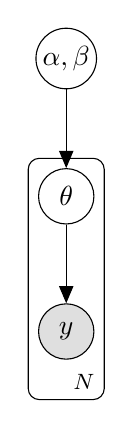
\begin{tikzpicture}
		\node[latent] (ab) {$\alpha,\beta$};
		\node[latent, below = of ab]  (theta) {$\theta$};
		\node[obs, below = of theta](y){$y$};
		
		\edge{ab}{theta};
		\edge{theta}{y};
		
		\plate{exp}{(theta)(y)}{$N$};
	\end{tikzpicture}
	\caption[Hierarchical binomial model bayes net]{Bayes net for hierarchical binomial model.  Note here that nodes with shading correspond to observed data, while nodes without shading are latent.}
	\label{bayesnet}
\end{figure}

Bayes nets can be used to do inference, and a literature of algorithms and methods exists for the purposes of doing so \cite{Bishop2006pattern,koller2009probabilistic}.  Here, and in subsequent writings, I will use them solely for economy of thought when describing models.


\subsubsection{Model Assessment}

Once a model is specified, and the posterior for the parameters obtained, the model fit, not only to the data but also to the practitioner's substantive knowledge, must be assessed.  

Since the result of a Bayesian analysis is a posterior distribution of the model parameters, it is easy to simulate data from the data generating process.  Let $ y $ be observed data, and $ \theta $ be a vector of (hyper)parameters for the model.  Denote $ \tilde{y} $ as replicated data from the data generating process, or as Gelman writes, ``data that we \textit{would} have seen tomorrow if the experiment that generated $ y $ today were replicated with the same model and the same value of $ \theta $ that produced the observed data" \cite[page~145]{gelman2013bayesian}.  Then the distribution of the replicated data conditioned on the observed data is 
%
\begin{equation}\label{PPD}
	p(\tilde{y} \vert y) = \int p(\tilde{y} \vert \theta) p(\theta \vert y) \, d\theta  \>.
\end{equation}
%
The distribution in \cref{PPD} is called the \textit{posterior predictive distribution}.  It stands to reason that if the model fits the data well, then observed data should look plausible under the posterior predictive distribution.  Simulated data sets are generated from \cref{PPD} and are compared to the observed data.  Any systematic differences between observed and simulated may point to areas in which the model can be improved.

Aspects of the observed data can be summarized into a \textit{test quantity} which is then compared against replicated data. This is usually some summary statistic of the observed data. Tail area probability computations can be used to quantify  the observed data's departure from the posterior predictive simulations.  If $ T(y) $ is a test quantity, then the tail area probability is $ P(T(\tilde{y}) > T(y) ) $.  This is similar to the Frequentist p-value.


\subsubsection{Markov Chain Monte Carlo \& Modern Methods}

The integrals in Bayesian statistics quickly become intractable when considering unusual models or relaxing assumptions for simple models.  Consequently, computational methods have been developed to aid in fitting models.  The result is the ability to sample from the posterior distribution without having to know the exact analytical form of the posterior density.

The suit of computational methods for sampling from the posterior are called \textit{Markov Chain Monte Carlo} (MCMC) methods.  These methods simulate Markov chains whose limiting distribution is the posterior distribution \cite{livingstone2016geometric}.  The most common MCMC methods for drawing  samples from the posterior are The Metropolis-Hastings Algorithm and Gibbs Sampling \cite{gelman2013bayesian,mcelreath2016statistical}.  Recently however, these algorithms have given way to more efficient algorithms, known as \textit{Hamiltonian Monte Carlo} (HMC) methods.  HMC is inspired by Hamiltonian mechanics. The posterior is idealized as a surface on which a particle of mass $ m $ rolls after being given a random position and momentum vector.  The geometry of the surface influences the movement of the particle, and thus influences the samples obtained.  HMC is a marvellously interesting method, spanning topics such as physics, numerical differential equations, and differential geometry.  The theory for HMC is quite dense, and more appropriate for a computer science department.  I refer interested readers to the following resources \cite{ gelman2013bayesian, livingstone2016geometric, mcelreath2016statistical,neal2011mcmc, hoffman2014no,betancourt2017conceptual}.

\subsubsection{Diagnostics for Hamiltonian Monte Carlo}

Provided the simulated Markov chain is geometrically ergodic, a law of large numbers and a central limit theorem exists for these Markov chains \cite{livingstone2016geometric, betancourt2017robust}, thus allowing users to be confident in inferences made from the samples obtained.  General conditions under which the chain is and is not geometrically ergodic exist \cite{livingstone2016geometric}, but verification of these properties for applied problems is not usually done analytically.  Instead, diagnostics are used to assess the reliability of inferences from the Markov chains.

The first diagnostic most applied Bayesians are introduced to is called the potential scale reduction factor, or Gelman-Rubin diagnostic, or $ \rhat$.    In MCMC and HMC, several chains are usually initialized and allowed to run for sufficiently long to as to (hopefully) arrive at their stationary distribution.  If geometric ergodicity holds, then all chains should arrive at the same stationary distribution, and thus be exploring the same space.  The Gelman-Rubin diagnostic  measures how well the chains are exploring the space by comparing the within chain variance to the between chain variance \cite{gelman2013bayesian}.  In practice, $ 1.1<\rhat $ indicates a problem with the chains, and inference should not be made from the samples drawn \cite{betancourt2017robust}.

Another diagnostic is the effective sample size, $ n_{eff} $.  The Markov chains generate correlated samples, not completely random samples, so using existing theories of convergence of functions of random variables are inappropriate.  Effective sample size is heuristic to measure how close the samples are to being independent.  Effective sample size is defined as
%
\[ n_{eff} = \dfrac{n}{1+ 2\displaystyle\sum_k \rho(k)} \>. \]
%
Here, $ \rho(k) $ is the lag-$k$ within chain correlation \cite{gelman2013bayesian,kass1998markov}.  If the chains are autocorrelated, then $n_{eff} <n$, and if the chains are completely independent $n_{eff} = n$. If chains are highly correlated, then $n_{eff} \ll n$, and inferences made from the samples should be avoided because of the bias the correlation would impart.
	\subsection{Pharmacokinetics \& Pharmacodynamics}

In this section, I describe pharmacokinetic and pharmacodynamic theory as it will be used in the proposed research.  I will explain aspects of both pharmacokinetic and pharmacodynamic models, and how the two are related.  One and two compartment model(s) for pharmacokinetics will be constructed and interpreted.


\subsubsection{Pharmacokinetics v. Pharmacodynamics}

The phases between drug administration and emergence of the desired effect can be broadly placed into one of two areas of study.  The area of study which is concerned with relationship between dose administration and achievement of particular concentrations in the body is known as \textit{pharmacokinetics}, while the area of study concenred with the arrival of the drug at it's site of action, the onset of the desired effect, as well as the magnitude and duration of that effect is known as  \textit{pharmacodynamics} \cite{rosenbaum2016basic}.  

\subsubsection{A One Compartment Pharmacokinetic Model}

To analyze the time course of drug concentrations in various parts of the body, compartmental models are often used.  These models posit that the body (or relevant organs/systems of the body) is comprised of compartments from which drug can flow in and out. The rates at which the drug can enter and exit each compartment are specified, and a differential equation for each compartment can be created and solved.

The simplest example of these models is the one compartment pharmacokinetic model.  A bolus dose of a drug is administered to the patient and the drug is absorbed from the gut into the blood.  Here, the gut and the blood form two compartments, but we are not usually interested in concentrations of drug in the gut, and so we usually focus only on the concentration of drug in the blood (hence, one compartmental model).  A visual representation of this model is shown in \cref{compartmental_model}.

\begin{figure}[h!]
	\centering
	
	\tikzstyle{int}=[draw, fill=white, minimum size=2em]
	\tikzstyle{init} = [pin edge={to-,thin,black}]
	
	
	\begin{tikzpicture}[node distance=2.5cm,auto,>=latex']
	
	
	\node [int] (a) {$G$};
	\node (b) [left of=a,node distance=2cm, coordinate] {a};
	\node [int] (c) [right of=a] {$C$};
	\node [coordinate] (end) [right of=c, node distance=2cm]{};
	\path[->] (a) edge node {$k_a$} (c);
	\draw[->] (c) edge node {$k$} (end) ;
	\end{tikzpicture}
	\caption{A compartmental diagram for a one compartment pharmacokinetic model.}
	\label{compartmental_model}
\end{figure}

In this diagram, $ G $ is the compartment for the gut, and $ C $ is the compartment for the blood.  Both $ G $ and $ C $ represent the concentrations of drug in gut and blood respectively.  The drug leaves the gut ($ G $) and enters the blood ($ C $) at rate $ k_aG $.  The drug is then excreted from the body at rate $ kC $.  The system can be written as a differential equation, namely,
%
\begin{alignat*}{3}
	\dfrac{dG}{dt} &= -k_aG \>, \quad  &&G(0) = \dfrac{D}{V} \\
	\dfrac{dC}{dt} &= k_aG - kC \>,   \quad  &&C(0) = 0
\end{alignat*}
%
Here, $D>0$ is the dose size and $V>0$ is the volume of the gut.  It can be shown that the solution for the concentration of drug in the blood at a given time is 

\begin{equation}\label{onecompartment_PKPD}
	C(t) = \dfrac{D}{V}\dfrac{k_a}{k_a - k}\Big(e^{-k_at} - e^{-kt}\Big) \>.
\end{equation}

\begin{figure}[h!]
	\centering
	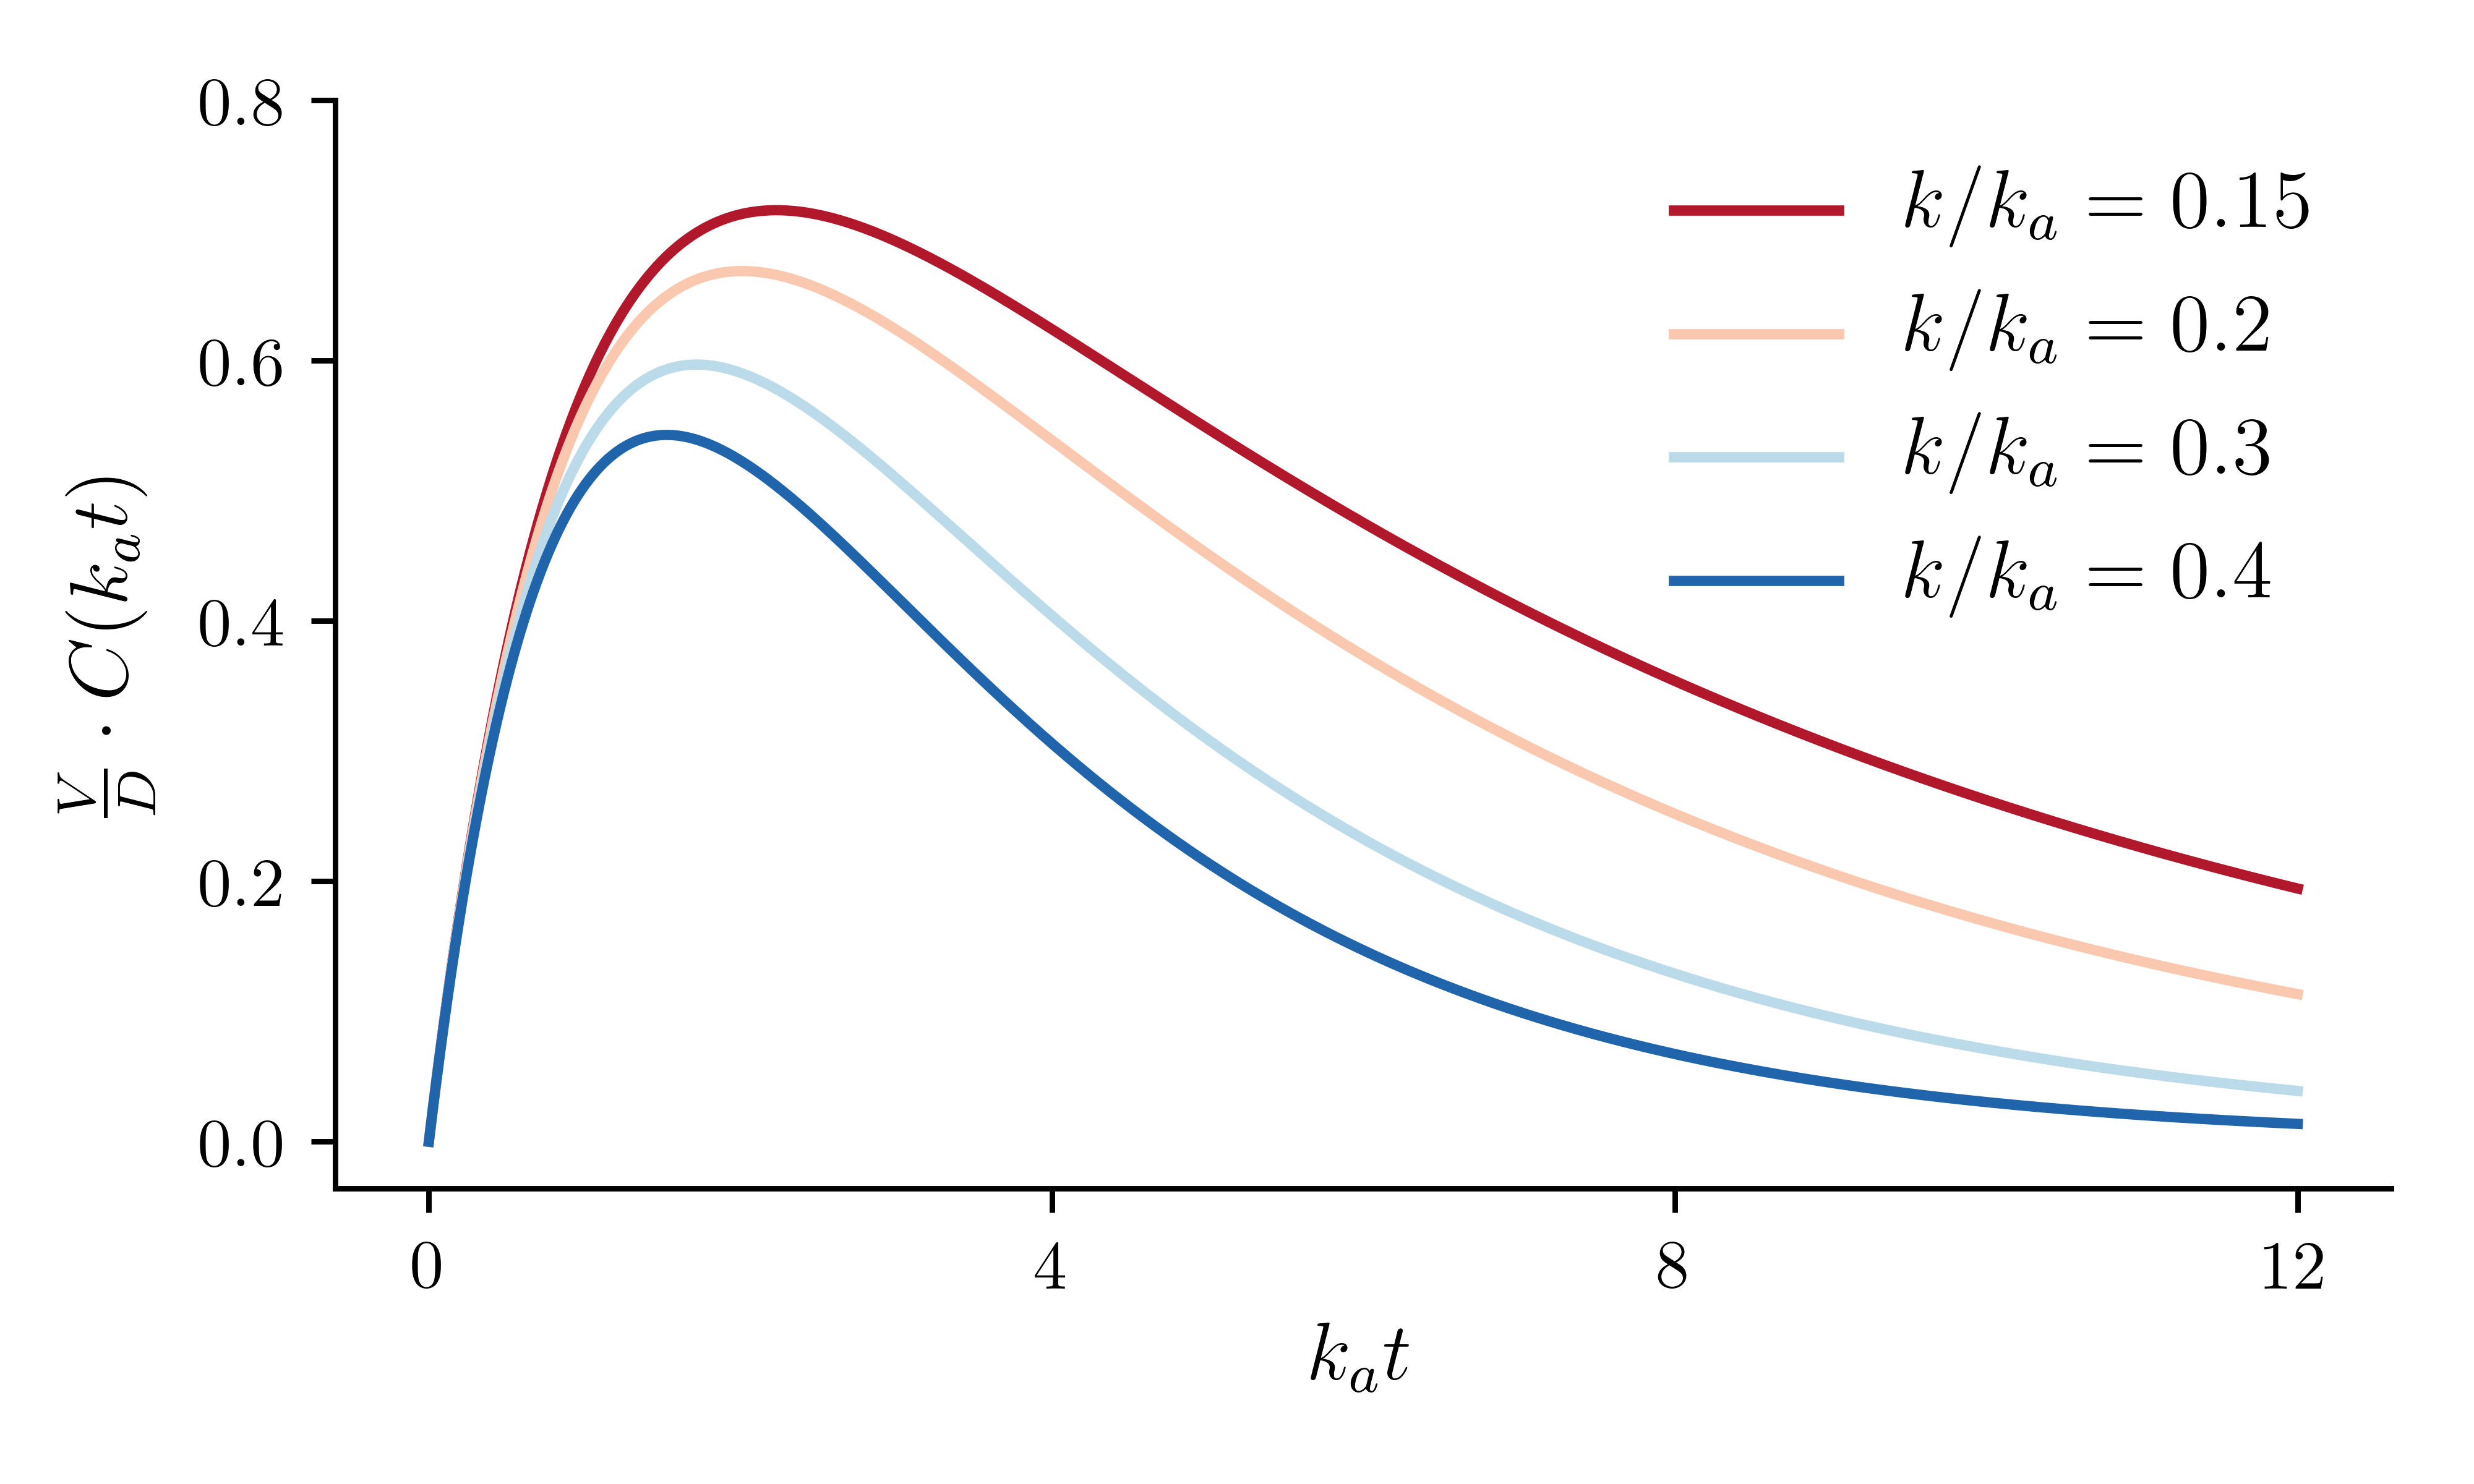
\includegraphics{Figures/pkcureves.png}
	\caption{Plots of \cref{onecompartment_PKPD} under various parameterizations.  Holding $D/V$ constant and examining various values of $k/k_a$ leads to curves shown.  The time scale has also been altered so as to account for varying rates of drug influx/outflux.  This process is called \textit{non-dimensionalization}, and is often used in the analysis of dynamical systems.  We see that as $\frac{k}{k_a} \rightarrow 1^-$, the maximum concentration of drug in the blood shrinks, and the drug exists the body much faster.}
	\label{fig:pkcureves}
\end{figure}


\subsection{A Two Compartment Pharmacokinetic Model}	
	\subsection{Reinforcement Learning}

In this section, I describe concepts from reinforcement learning as they will be used in the proposed research.  Reinforcement learning is a sub field of artificial intelligence used in optimal decision making. The term "reinforcement" indicates that the algorithms learn from actions which are rewarded, with favourable actions being rewarded according to their benefit \cite{sutton2011reinforcement}.  Thus, the algorithms learn through positive/negative "reinforcement".  The actions and their reward are not typically know \textit{a priori}, and so these algorithms are said to "learn from experience".  In particular, sequential decision making,Markov decision processes, and optimal policies, and goals for learning algorithms are discussed.

\subsubsection{Formalization of Sequential Decision Making}

Reinforcement learning idealizes the algorithm (or entity doing the decision making) as an \textit{agent} continually interacting with a \textit{environment}.  At a sequence of discrete time steps  (${ t =1, 2 \dots, n} $), the agent evaluates the current \textit{state} of the environment $ S_t $, decides on an \textit{action} ($ A_t $), receives a \textit{reward} for that action $ R_{t+1} $, and then finds itself in a \textit{new state} ($ S_{t+1} $).  This sequence of state, action, reward, new state is called a \textit{trajectory} \cite{sutton2011reinforcement,lizotte2017reinforcement}.  Here, 

The set of all states in which the agent may find itself in ($\mathcal{S}$), the set of all actions which the agent may make ($\mathcal{A}$), the set of rewards given to the agent ($ \mathcal{R} $), and the distribution of new states ($ P $) the agent could find itself in if it takes action $ a_t $ in stats $ s_t $ for a \textit{Markov decision process} (MPD) \cite{sutton2011reinforcement,lizotte2017reinforcement}.

\begin{figure}[h!]
\centering
	
\tikzstyle{block} = [rectangle, draw, 
text width=8em, text centered, rounded corners, minimum height=4em]

\tikzstyle{line} = [draw, -latex]
\tikzstyle{block} = [rectangle, draw, 
text width=8em, text centered, rounded corners, minimum height=4em]

\tikzstyle{line} = [draw, -latex]

\begin{tikzpicture}[node distance = 6em, auto, thick]
\node [block] (Agent) {Agent};
\node [block, below of=Agent] (Environment) {Environment};

\path [line] (Agent.0) --++ (4em,0em) |- node [near start]{Action $A_t$} (Environment.0);
\path [line] (Environment.190) --++ (-6em,0em) |- node [near start] {New state  $S_{t+1}$} (Agent.170);
\path [line] (Environment.170) --++ (-4.25em,0em) |- node [near start, right] {Reward $R_{t}$} (Agent.190);
\end{tikzpicture}

\caption{Pictorial representation of the learning process.  At the present state $ S_t $, the agent makes action $ A_t $.  The action is rewarded with $ R_t $ and the agent finds itself in a new state $ S_{t+1} $.  The process repeats and forms a trajectory of $ {S_t,A_t,R_t,S_{t+1}, A_{t+1}, R_{t+1}, S_{t+2}, \cdots} $.  }
\label{RL_diagram}
\end{figure}


\subsubsection{Policies}

The agent will choose actions based on a \textit{policy}.  A policy, $ \pi $, is a function which maps the set of states to the set of actions  
%
\begin{equation}\label{key}
\pi : \mathcal{S} \rightarrow \mathcal{A}\>.
\end{equation}
%
Associated with a particular trajectory is a \textit{return}, $ \sum_t R_t \gamma^t $, where $ \gamma $ is constant and $ 0 < \gamma < 1 $.  The environment is assumed to be stochastic, thus the return are random quantities. Let $ \mathbf{\Psi}_{\pi,s} $ be a random variable for the return following policy $ \pi $ in state $ s $.  The \textit{value} of a policy is the expected return of that policy, $V_{\pi}(s) =  \mathbb{E}(\mathbf{\Psi}_{\pi,s}) $ \cite{lizotte2017reinforcement}.  A policy is said to be \textit{optimal} if the value of the policy is larger than all other policies under all possible states.  Mathematically, a policy $ \pi^* $ is optimal if and only if $ V_{\pi}(s)  \leq V_{\pi^*}(s) \> \forall \pi, \forall s\in \mathcal{S}  $.


\subsubsection{Goals for Learning}
Different algorithms seek to learn different aspects of the problem at hand.  Temporal difference learning seeks to compute a value function given by experience generated by a policy, while Q-learning attempts to learn an optimal policy given the agent's experience \cite{lizotte2017reinforcement}.  The details of these algorithms are beyond the scope of this proposal.	
	
	
	
	\newpage
	\addcontentsline{toc}{section}{\textbf{References}}
	\bibliography{Sections/ODEs/ODEs_bib,Sections/Bayes/Bayes_bib,Sections/PKPD/PKPD_bib}
	\bibliographystyle{unsrt}

\end{document}